\documentclass[oneside]{book}
\usepackage[utf8]{inputenc}
\usepackage{fancyhdr}
%\usepackage{listings}
\usepackage[document]{ragged2e}
\usepackage{lastpage}
\usepackage{circuitikz}
\usepackage{amsmath}
\usepackage{amssymb}
\usepackage{mathrsfs, amsmath}
\usepackage{amsfonts}
\usepackage{amsthm}
\usepackage{caption}
\usepackage{subcaption}
\usepackage{tcolorbox}
\usepackage{cancel}
\usepackage{nccmath}
\usepackage{wrapfig}
\usepackage{hyperref,lipsum}
\usepackage[export]{adjustbox}
%\usepackage{fullpage}
\usepackage{geometry}
\usepackage{listings}
\usepackage{textcomp}
\pagestyle{fancy}
\fancyhf{}
\fancyhead[L]{\leftmark} % Chapter name at the left header
\fancyhead[R]{\thepage} % Page number at the right header
\renewcommand{\chaptermark}[1]{\markboth{#1}{}}
\hypersetup{
    colorlinks=true,
    linkcolor=blue,
    filecolor=magenta,      
    urlcolor=cyan,
    pdftitle={Overleaf Example},
    pdfpagemode=FullScreen,
    }
\begin{document}
\begin{titlepage}
\centering
{\bfseries\Huge Indian Institute of Technology Hyderabad\par}


\vfill
\noindent
{\bfseries\Huge Elektronica Club  \par}
\bigskip%Título
\vspace{0.5cm}

{\bfseries\Large Signal Processing\par}
\vspace{0.5cm}
\noindent
\vfill
{\Large K Rahul\par}
{\Large ee23btech11027 \par}
\vfill
\end{titlepage}
\setcounter{page}{0}
\newpage
\tableofcontents
\newpage
\Large

\chapter{Introduction} \label{Chapter-1}
A Signal is a sequence of values that conveys information about a phenomenon.
It can be physical, representing a physical quantity that varies over time or
space, or abstract, representing information in a coded or symbolic form. Some
examples include, Neural Signals, Stock Market Movement, Seismic Waves and
many more in various domains! \\
\bigskip
Signal Processing is the analysis, manipulation, and interpretation of signals to
extract useful information, enhance quality, or transform them for different
applications. It encompasses a wide range of techniques and applications, often
involving the use of mathematical algorithms to process the signals.\\
\bigskip
A Signal can be represented in two domains - Time Domain and Frequency
Domain and the whole heart of Signal Processing is a mathematical operation
known as Fourier Transform which transforms the signal from one domain to
another.

\newpage
\chapter{What is the Fourier Transform?}
Naively speaking, a Fourier transform is simply a way to express signal in time domain as a combination of sinusoids(more specifically, complex exponentials). The advantage of being able to express a signal in these terms becomes apparent upon realizing that a large number of systems dealt with are LTI systems and the complex exponential, upon sbeing subjected to an LTI system, shows the following property:
\begin{align}
    e^{st} \rightarrow H(s)e^{st}, s \in \mathcal{C}
\end{align}
Where $H(s)$ is a complex amplitude factor. The important thing to note is that the output of the LTI system has the same complex exponential as the input of the LTI system, with only an amplitude factor.\\
The Fourier Transform of a signal in continuous time is given as 
\begin{align}
    X(f) = \int_{-\infty}^{+\infty} x(t)e^{-j2\pi f t} dt \label{CTFT}
\end{align}
The inverse operation is given as
\begin{align}
    x(t) = \int_{-\infty}^{+\infty}X(f)e^{j2\pi ft}df \label{Inverse_CTFT}
\end{align}
Most modern work on frequency domain analysis is done on computers, that cannot process such real continuous signals directly, hence small "samples" of $x(t)$ are taken at regular intervals of time .Let the sampling time be $T_s$, then the value of $x(t)$ can be found at $x(t = nT_s)$, where $n$ is an integer. This, hence, can be considered to form a sequence $x[n]$, where $x[n] = x_a(t = nT_s)$, where $x_a(t)$ is the analog signal upon which sampling takes place. \\
\bigskip
The Fourier Transform on such a sampled signal is given as
\begin{align}
    X(f) = \sum_{n = -\infty}^{\infty} x[n] e^{-j2\pi f n} \label{DTFT}
\end{align}
The equation \eqref{DTFT} is also continuous and hence they need to be sampled as well to render it useful for a computer. Without going into too much detail, this sampled version of \eqref{DTFT} is called the DFT(Discrete Fourier Transform), and the fast way of evaluating this DFT is called the FFT(Fast Fourier Transform) Algorithm.

This transform helps in understanding the nature of a signal in frequency analysis and hence is useful for such kind of analysis, like in filtering, for example.

\newpage
\chapter{Convolution in MATLAB}
Convolution is a process central to the idea of LTI systems. Given the impluse response of an LTI system $h[n]$\footnote{From now on, all computation is to be done on a computer, so all concepts would exclusively be dealt in the discrete domain.}, the output $y[n]$ for any input signal $x[n]$ is given as
\begin{align}
    y[n] = \sum_{k\; = -\infty}^{+\infty}x[n]h[n]
\end{align}
In the context of computer languages(like Python or MATLAB), the signals $x[n]$ and $h[n]$ are denoted as arrays(or lists, in Python). The code is implemented \href{https://github.com/HarryNyquist/Elektronica/blob/main/Signal_Processing/Convolution/convolution_sum.m}{\underline{\textbf{here}}}, in MATLAB, under the function \verb|convolution_sum|. \\ \bigskip
If the length of the array $x[n]$ and $h[n]$ are $a$ and $b$ respectively, the length of the output array $y[n]$ is $a + b - 1$.
\chapter{Noise Removal from Speech Signal}
This problem statement deals with filtering techniques. A speech signal is given in the form of beeps, and these beeps must be eliminated to produce a clean speech signal. \\ \bigskip

The sound speech with beeps is \href{https://github.com/HarryNyquist/Elektronica/blob/main/Signal_Processing/Audio_Filtering/Noise_Removal.wav}{\underline{\textbf{here}}}, and the filtered sound with only speech voice is \href{https://github.com/HarryNyquist/Elektronica/blob/main/Signal_Processing/Audio_Filtering/Filtered_output.wav}{\underline{\textbf{here}}}. The code used in carrying out the filtering is given \href{https://github.com/HarryNyquist/Elektronica/blob/main/Signal_Processing/Audio_Filtering/Bandpass_filter.m}{\underline{\textbf{here}}}.\\
All these codes can be found at \href{https://github.com/HarryNyquist/Elektronica/blob/main/Signal_Processing/Audio_Filtering/Bandpass_filter.m}{\underline{\textbf{in this repository directory}}}
The FFT of the initial unfiltered noise was first taken and plotted.
\begin{figure}[htbp]
    \centering
    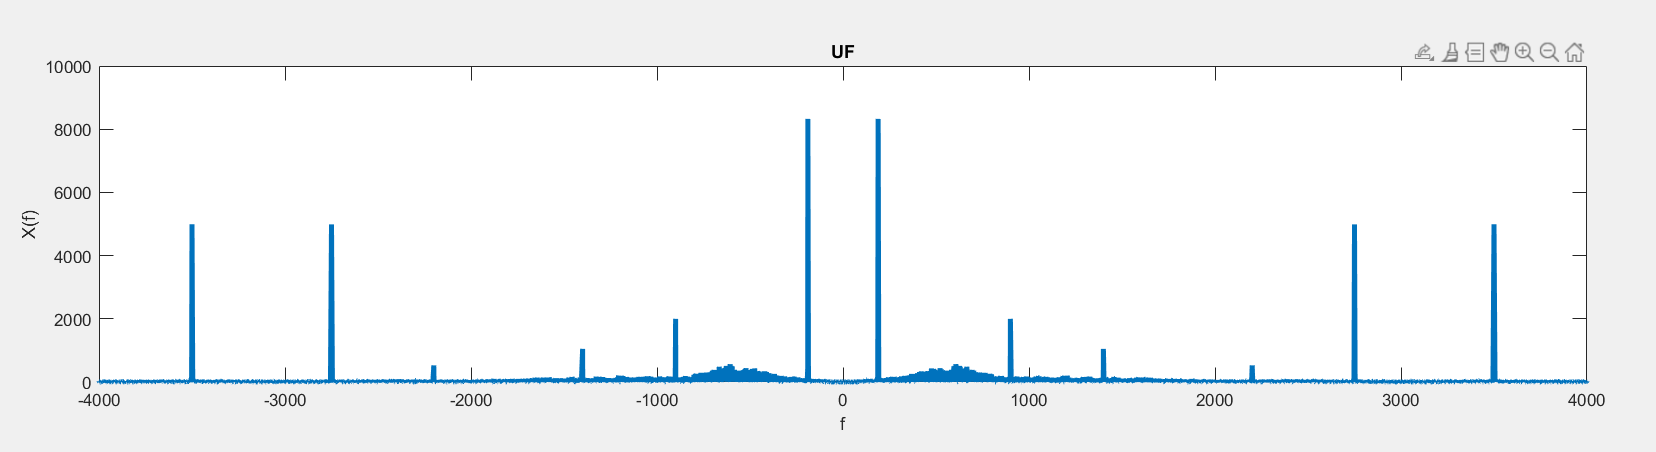
\includegraphics[width=1\textwidth]{figs/Unfiltered_Audio_Signal.png}
    \caption{FFT of unfiltered Audio Signal}
\end{figure}
\newpage
After identifying the ranges of frequencies that caused the beeps, they were removed a combination of a Butterworth bandpass filter and Butterworth bandstop filter, after which a clear audio signal was recovered. \\
The FFT of the clear audio signal is given below.
\begin{figure}[htbp]
    \centering
    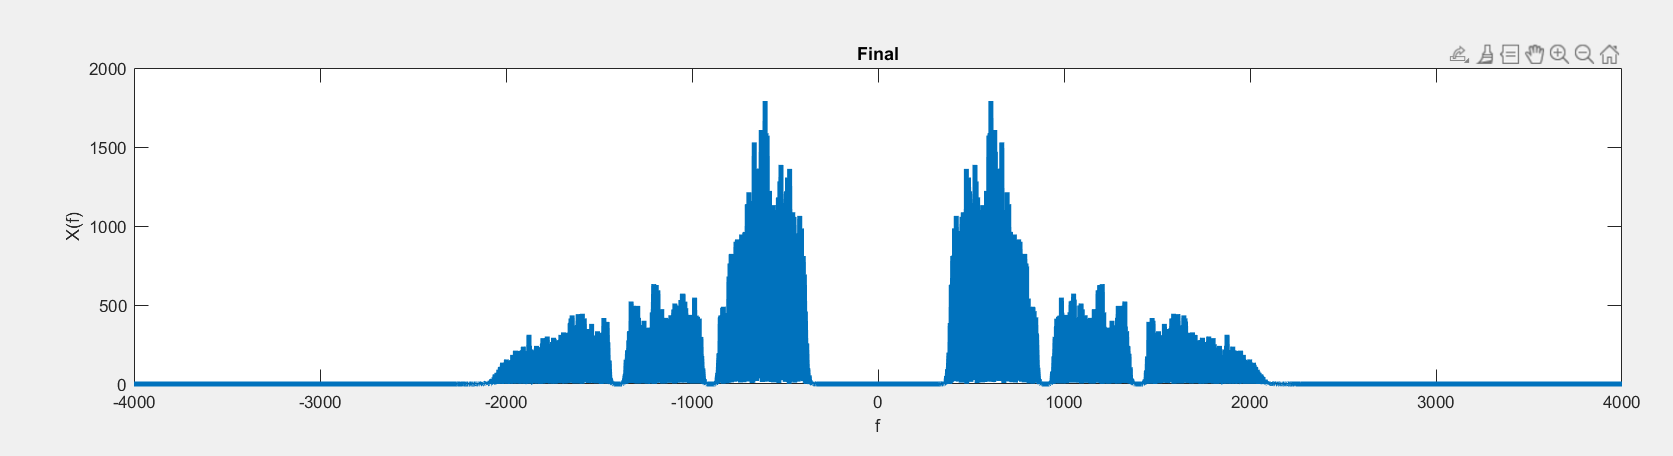
\includegraphics[width=1\textwidth]{figs/Filtered_Audio_Signal.png}
    \caption{FFT of filtered Audio Signal}
\end{figure}
\\ \bigskip
The reason why a normal Brickwall bandpass type of filter, that sets all frequencies $|f|$ such that $|f| > |f_{c1}|$ and $|f| < |f_{c2}|$ to zero cannot really work is that the FFT is just a sampled version of the DTFT. This means that upon extrapolation of the points of the FFT, a ripple would be formed in the DTFT when the FFT bins are set to zero. Hence, it would not cause the type of filtering expected from a Brickwall filter. One way to circumvent this would be to set the sampling frequency $F_s$ to be very large, as the FFT at $F_s \rightarrow \infty$ is identical to the DTFT. However, this is quite impractical. Another solution might be to use a window function and convolve with the $sinc$ function in that limited window, but they probably give some other side effects that haven't been explained here.

\end{document}